\newpage
\section{RESULTS AND ANALYSIS}

This part is dedicated to the final performance appraisal of the proposed automatic alignment of the antennas solution. Performance analysis involves simulation results and hardware testing results to investigate the RL controller’s performance from three different viewpoints, including expected performance, simulation performance, and actual performance on embedded systems. Analysis results will be shown in table format, graphs, and comparisons between convergence time, received signal strength, movement effort, and repeatability.

\subsection{Simulation Results Summary}

Simulation was the first validation step where all approaches could be compared with the same path loss, directional gain, and noise values. Simulation results showed that there were trade-offs between the three approaches. Exhaustive search would guarantee the highest accuracy with the longest time. Hill climbing was a fast approach with a tendency to fall into local maxima.

\vspace{0.5cm}
\begin{table}[H]
\centering
\caption{Summary of Simulation Performance}
\label{tab:simulation_summary_final}
\renewcommand{\arraystretch}{1.35}
\begin{adjustbox}{width=\textwidth}
\begin{tabular}{|
>{\raggedright\arraybackslash}p{2.7cm}|
>{\raggedright\arraybackslash}p{2.2cm}|
>{\raggedright\arraybackslash}p{2.3cm}|
>{\raggedright\arraybackslash}p{2.1cm}|
>{\raggedright\arraybackslash}p{2.1cm}|
>{\raggedright\arraybackslash}p{2.4cm}|}
\hline
\textbf{Method} & \textbf{Best RSSI (dBm)} & \textbf{Conv. Time (s)} & \textbf{Actuator Steps} & \textbf{RSSI Samples} & \textbf{Robustness} \\
\hline
Exhaustive scan & $-30.14$ & 67.68 & 945 & 18{,}900 & Very high \\
\hline
Hill-climbing & $-32.13$ & 6.51 & 39 & 780 & Low to moderate \\
\hline
RL (Q-learning) & $\mathbf{-30.82}$ & $\mathbf{5.51}$ & 25 & 500 & High \\
\hline
\end{tabular}
\end{adjustbox}
\end{table}

\begin{figure}[H]
\centering
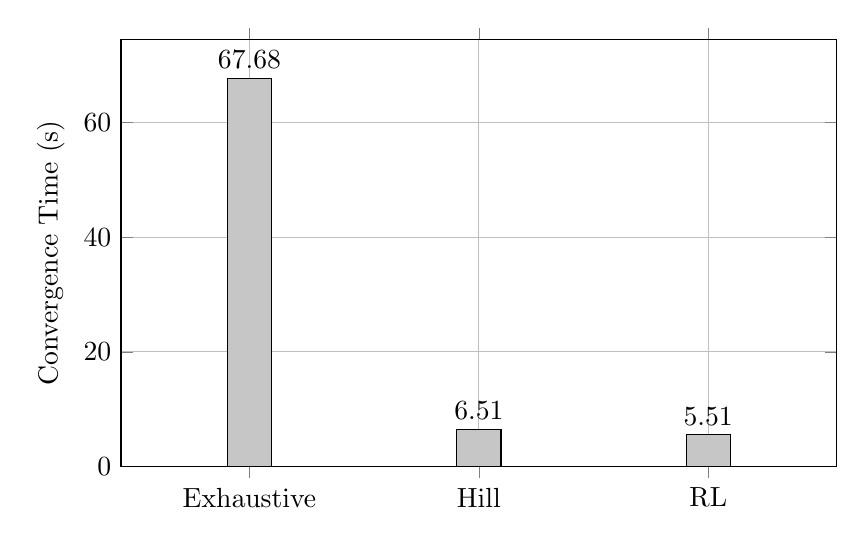
\begin{tikzpicture}
\begin{axis}[
    ybar,
    bar width=16pt,
    width=0.88\textwidth,
    height=7cm,
    ymin=0,
    ylabel={Convergence Time (s)},
    symbolic x coords={Exhaustive,Hill,RL},
    xtick=data,
    nodes near coords,
    nodes near coords align={vertical},
    enlarge x limits=0.28,
    grid=major
]
\addplot[fill=gray!45] coordinates {(Exhaustive,67.68) (Hill,6.51) (RL,5.51)};
\end{axis}
\end{tikzpicture}
\vspace{0.2cm}
\caption{Convergence time comparison in simulation}
\label{fig:sim_convergence_chart}
\end{figure}

Figure~\ref{fig:sim_convergence_chart} demonstrates how much time overhead is incurred by the exhaustive scanning process in the simulated setting. Both the hill-climbing and reinforcement learning (RL) algorithms show significantly faster convergence rates; in particular, RL demonstrates this characteristic without losing the ability to find the RSSI maximum and shows improved robustness to changing the starting position.

\subsubsection{Exhaustive Scanning}
The procedure resulted in finding the global maximum value of RSSI, which equals $-30.14$~dBm for the angle $(\theta_{\text{pan}}, \theta_{\text{tilt}}) =
(88^{\circ}, 90^{\circ})$. Hence, we can conclude that in the current setup, the simulation environment and antenna radiation model have led to the presence of the global optimum point that can be discovered via exhaustive search.

Nonetheless, reaching the optimal state required 945 steps and 18,900 RSSI evaluations, which amounts to 67.7 seconds of convergence time in the simulated setup. As can be seen from the large number of mechanical actions and RSSI evaluations, the exhaustive scanning method is quite inefficient and cannot be recommended for any practical implementation due to its high computational cost.

In other words, exhaustive scanning provides a reference for alignment performance while being impractical for real-world deployment.

Figure~\ref{fig:exhaustive_rssi} illustrates the RSSI variation observed across a full
angular sweep.

\begin{figure}[H]
\centering
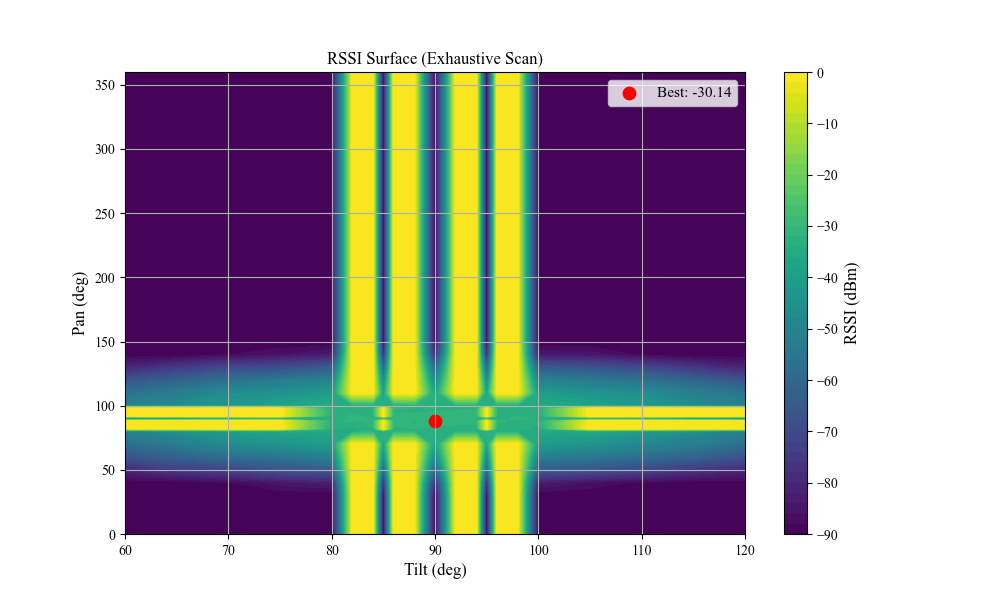
\includegraphics[width=1\textwidth]{images/Figure_1.png}
\caption{RSSI Variation During Exhaustive Scanning}
\label{fig:exhaustive_rssi}
\end{figure}

\subsubsection{Hill Climbing}

The hill-climbing approach was evaluated through a local greedy search model, where pan and tilt movements of $2^{\circ}$ were used for incremental updates to obtain maximum RSSI improvement. An average of 20 RSSI readings were taken per orientation setting, and a patience-based criterion was incorporated to stop the search process when no further improvements were possible.

With starting points that are close to the global optimum, the convergence speed was found to be very fast. For instance, when starting at an orientation of $(40^{\circ}, 70^{\circ})$, hill climbing achieved nearly optimal orientations of $(90^{\circ}, 86^{\circ})$ with RSSI values of $-32.13$~dBm. within only 39 actuator movements, which took 780 RSSI readings, amounting to about 6.51 seconds of convergence time. The convergence time required by the hill climbing algorithm is approximately one order of magnitude faster than the exhaustive scanning technique, yet achieving similar alignment performance.

\begin{figure}[H]
\centering
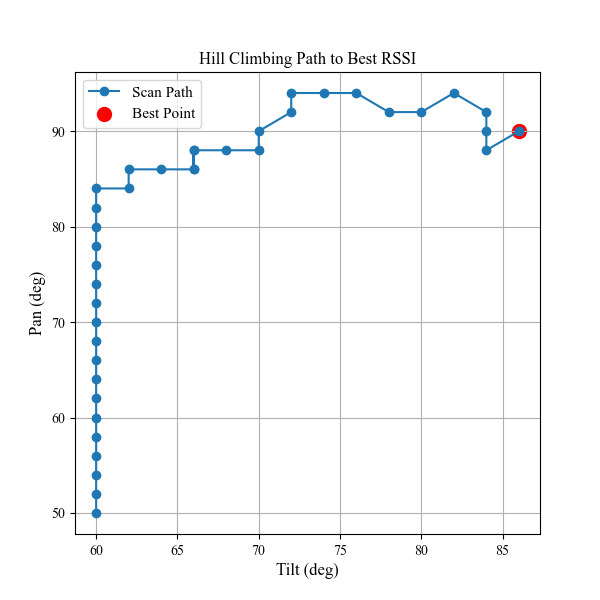
\includegraphics[width=0.9\textwidth]{images/Figure_2.png}
\caption{Path Traced During Hill Climbing}
\label{fig:hill_climbing_path}
\end{figure}

\begin{figure}[H]
\centering
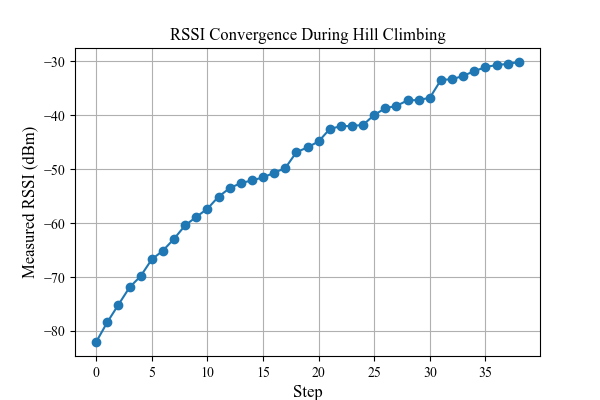
\includegraphics[width=0.8\textwidth]{images/Figure_3.png}
\caption{RSSI Variation During Hill Climbing}
\label{fig:hill_rssi}
\end{figure}

On the other hand, it showed strong dependency on initialization. When initializing from an unfavorable orientation point of $(150^{\circ}, 70^{\circ})$, the local search process got trapped in a suboptimal region and stopped within the first iteration with RSSI of $-90$~dBm. Such behavior is typical of greedy local search algorithms since there is no way for them to escape their local maxima regions.

\begin{figure}[H]
\centering
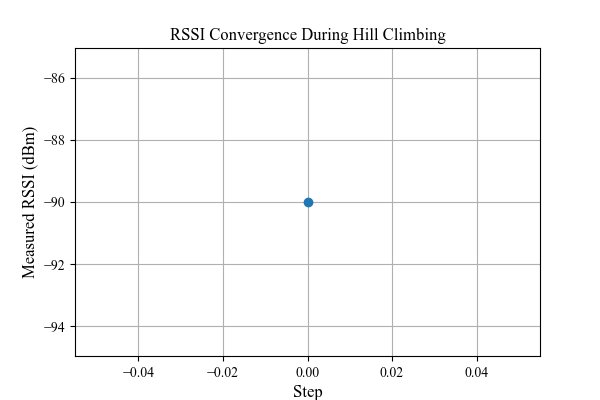
\includegraphics[width=1\textwidth]{images/Figure_6.png}
\caption{Unconverged RSSI Variation During Hill Climbing}
\label{fig:hill_climbing_path_unconverged}
\end{figure}

\newpage
\subsubsection{Reinforcement Learning}
The reinforcement learning (RL)-based alignment procedure was implemented using an agent based on the Q-learning algorithm, trained in the identical simulated antenna environment used during the exhaustive and hill climbing tests.

\begin{figure}[H]
\centering
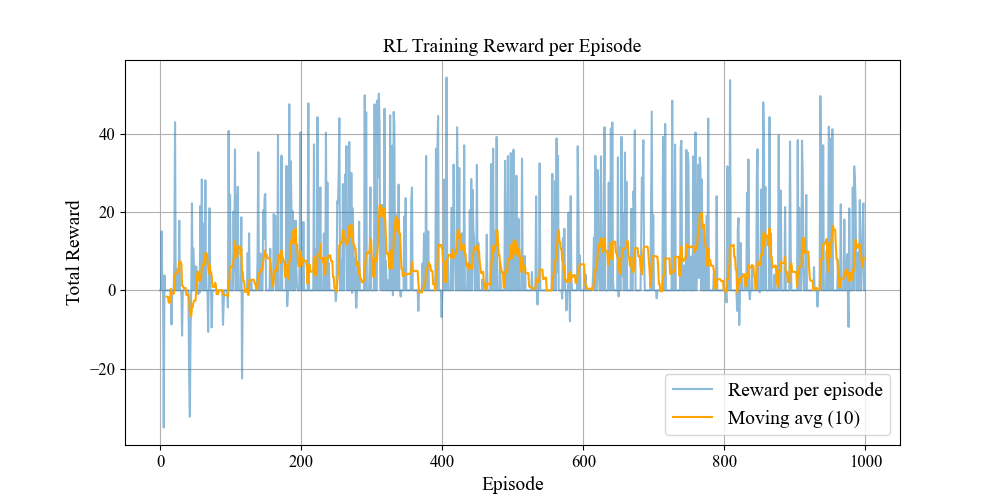
\includegraphics[width=1\textwidth]{images/Figure_7.png}
\caption{RL Training Reward Per Episode}
\label{fig:training_reward_rl}
\end{figure}

\begin{figure}[H]
\centering
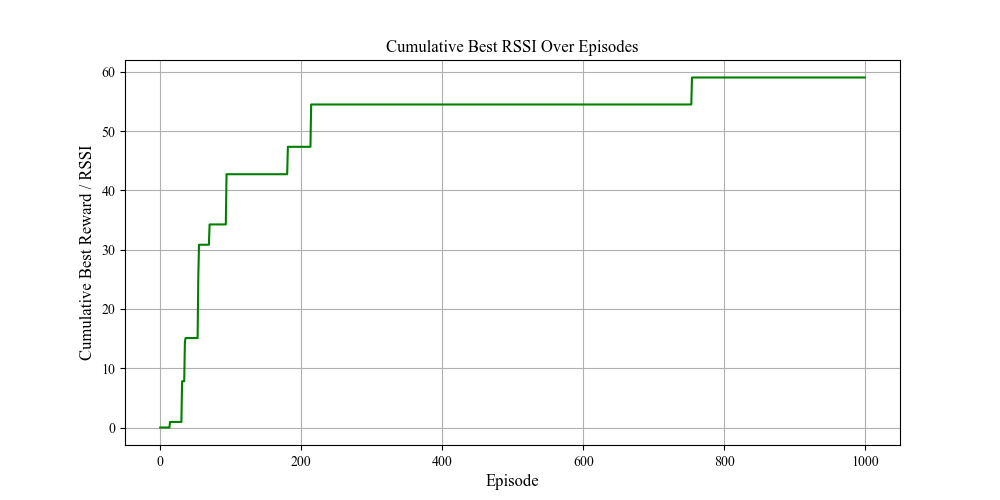
\includegraphics[width=1\textwidth]{images/Figure_8.png}
\caption{Cumulative Best RSSI Over Episodes}
\label{fig:cumulative_rl_path}
\end{figure}

Once the training phase converged, the resulting Q-table was frozen and used to evaluate the model in inference mode. The evaluation was performed starting from various different orientations of the antenna within the entire pan/tilt search space. In all tested cases, the RL agent managed to converge towards the global RSSI maximum point without knowing anything about the optimal orientation beforehand.

The RL controller was able to reach RSSI levels comparable to those achieved by the exhaustive search method but at the cost of far fewer actuation steps and RSSI measurements. Unlike the hill climbing method, the RL agent proved capable of escaping unfavorable initial conditions and local optima thanks to its ability to learn state-action value representations.

The convergence process appeared to be more stable and smooth across a variety of start positions. After being trained, the agent was able to perform inference solely based on table lookups and greedy actions, making the latter process lightweight and appropriate for implementation on microcontrollers like the ESP32-S3.

\begin{figure}[H]
\centering
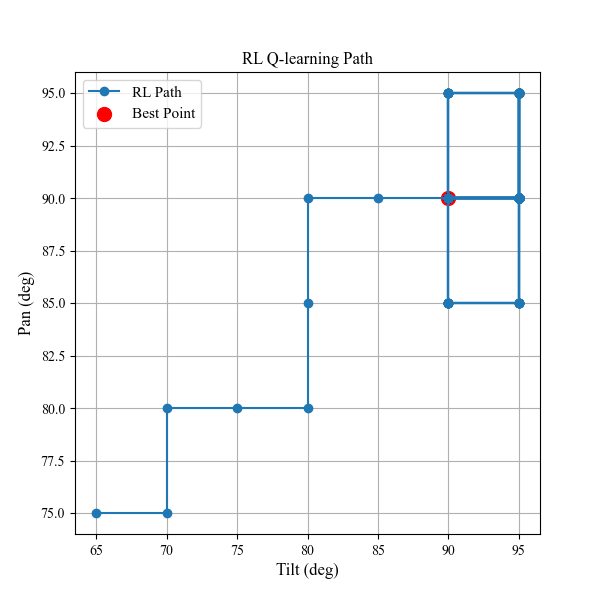
\includegraphics[width=0.9\textwidth]{images/Figure_9.png}
\caption{RL Q-Learning Path}
\label{fig:rl_rssi_convergence}
\end{figure}

\begin{figure}[H]
\centering
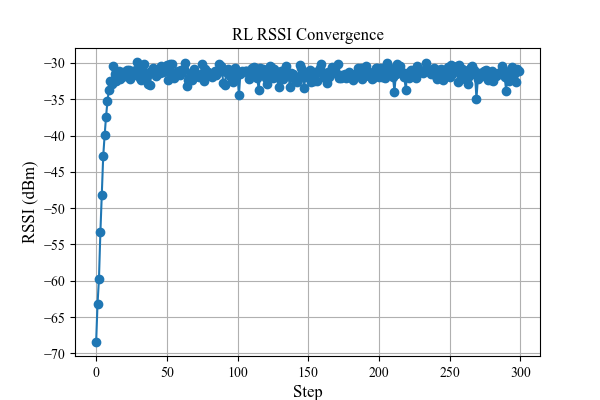
\includegraphics[width=1\textwidth]{images/Figure_10.png}
\vspace{0.15cm}
\caption{RL RSSI Convergence}
\label{fig:rl_rsssiconv}
\end{figure}

Overall, it can be concluded that the reinforcement learning approach provides a good balance between convergence speed, robustness to initialization, computational efficiency, and final RSSI performance in comparison with other approaches.